\section{Ablauf der Fahrzeugsteuerung} \label{hauptprogrammKapitel}
Damit die Fahrzeugsteuerung gestarten werden kann, muss die Datei \textit{fahrzeugsteuerung.php} ausgeführt werden. Obligatorisch für die Fahrzeugsteuerung ist die Abschnittsüberwachung (\textit{abschnittueberwachung.php}), welche vor dem Start der Fahrzeugsteuerung ausgeführt werden muss und auf deren Verwendung und Funktionsweise in Kapitel \ref{main_5} eingegangen wird. Der Aufbau dieses Kapitels orientiert sich an dem Ablauf der Fahrzeugsteuerung, welcher in Abbildung \ref{fig:hauptprogramm} schematisch dargestellt wird.
\begin{center}
\begin{figure}
\resizebox{1\textwidth}{!}{
\begin{tikzpicture}[node distance=0.7cm, auto,]
\node[punkt] (a) {Einbindung aller benötigten Dateien};
\node[below=of a, punkt] (b) {Einlesen von statischen und mehrfach verwendeter Daten aus der \textit{MySQL}-Datenbank in den Cache};
\node[below=of b, punkt](c) {Ermittlung aller Fahrzeuge im eingleisigen Netz und den zugehörigen Daten};
\node[below=of c, punkt](d) {Berechnung der Fahrtverläufe aller Fahrzeuge};
\node[right=of d, punkt](e) {Übermittlung der \Gls{echtzeitdaten} an die Fahrzeuge};
\node[right=of e, punkt](f) {Überprüfung nach neuen Fahrzeugen, Fahrplanänderungen, Fahrstraßenänderungen und Positionskalibrierung};
\node[above=of f, punkt](g) {Neuberechnung der Fahrtverläufe (falls notwendig)};
\draw [pil] (a) -- (b);
\draw [pil] (b) -- (c);
\draw [pil] (c) -- (d);
\draw [pil] (d) -- (e);
\draw [pil] (e) -- (f);
\draw [pil] (f) -- (g);
\draw [pil] (g.west) -- +(-0.5,0) -| (e.north);
\end{tikzpicture}
}
\caption{Ablauf der Fahrzeugsteuerung}
\label{fig:hauptprogramm}
\end{figure}
\end{center}
\subsection{Einlesen von statischen und mehrfach verwendeten Daten aus der \textit{MySQL}-Datenbank in den Cache} \label{main_1}
Die Fahrzeugsteuerung benötigt als Grundlage für viele Berechnungen Daten aus der \textit{MySQL}-Daten\-bank. Damit diese Daten nicht bei jeder Verwendung erneut aus der Datenbank geladen werden müssen und somit die Anzahl an Datenbank-Abfragen möglichst gering gehalten werden kann, werden die wichtigsten Daten beim Programmstart bzw. bei der ersten Verwendung in den Cache geladen (Code-Beispiel \ref{lst:cacheVars}). Beispielhaft zu nennen sind hierbei \textit{\$cache\-Infra\-Laenge} (Länge aller \acp{infra} in Metern), \textit{\$cache\-Haltepunkte} (zugehörige \ac{infra}e für alle Betriebsstellen und Richtung), \textit{\$cacheZwischenhaltepunkte} (zugehörige \acp{infra} für alle Zwischen-Betriebsstellen, die nur einem \ac{infra} zugeordnet sind), \textit{\$cache\-Gbt\-To\-Infra} (Zuordnung der \acp{infra} zu den GBT-Abschnitten) und \textit{\$cache\-Infra\-To\-Gbt} (Zuordnung der GBT-Abschnitte zu  den \acp{infra}n).
\begin{lstlisting}[caption={Initialisierung der Cache Variablen \textit{(fahrzeug\-steu\-e\-rung.php)}},captionpos=b,label={lst:cacheVars}]
// Statische Daten einlesen
$cacheInfranachbarn = createCacheInfranachbarn();
$cacheInfradaten = createCacheInfradaten();
$cacheSignaldaten = createCacheSignaldaten();
$cacheInfraLaenge = createcacheInfraLaenge();
$cacheHaltepunkte = createCacheHaltepunkte();
$cacheZwischenhaltepunkte = createChacheZwischenhaltepunkte();
$cacheInfraToGbt = createCacheInfraToGbt();
$cacheGbtToInfra = createCacheGbtToInfra();
$cacheFmaToInfra = createCacheFmaToInfra();
$cacheInfraToFma = array_flip($cacheFmaToInfra);
$cacheFahrplanSession = createCacheFahrplanSession();
$cacheSignalIDToBetriebsstelle = createCacheToBetriebsstelle();
$cacheFahrzeugeAbschnitte = createCacheFahrzeugeAbschnitte();
$cacheIDTDecoder = createCacheDecoderToAdresse();
$cacheDecoderToID = array_flip($cacheIDTDecoder);
$cacheAdresseToID = array();		// Filled with data in getAllTrains()
$cacheIDToAdresse = array();		// Filled with data in getAllTrains()
\end{lstlisting}
\subsection{Ermittlung der Session-Daten} \label{main_12}
In der \textit{MySQL}-Tabelle \textit{fahrplan\_session} sind alle Fahrplansessions aufgelistet und der aktuell gültigen wurde der Wert 1 in der \textit{status}-Spalte zugeordnet. Die Daten der gültigen Fahrplansession wurden bei dem Start der Fahrzeugsteuerung in dem Array \textit{\$cacheFahrplanSession} gespeichert und werden benötigt, um die Zeitdifferenz zwischen Real- und \Gls{simulationszeit} zu ermitteln. Dafür wird im ersten Schritt das Datum der \textit{sim\_startzeit} und \textit{sim\_endzeit}, welche die Start- und Endzeit (\Gls{simulationszeit}) der Simulation im \Gls{unix}-Format angeben, auf das aktuelle Datum der \Gls{realzeit} geändert und im zweiten Schritt mit der \Gls{realzeit} verglichen (Code-Beispiel \ref{lst:readTime}).

Das Datum der \Gls{simulationszeit} wird angepasst, damit auch Fahrplansessions ausgeführt werden können, die nicht dem aktuellen Datum der \Gls{realzeit} entsprechen. Für die Umwandlung des Datums werden die Zeiten mittels der Funktion \textit{getUhrzeit$($$)$}$^\ast$ in das \textit{hh:mm:ss}-Format umgewandelt und mit derselben Funktion wieder in das \Gls{unix}-Format zurück umgewandelt.

Für die Ermittlung der \Gls{realzeit} und der Zeitdifferenz zwischen Real- und \Gls{simulationszeit} wird die Funktion \textit{time$($$)$} aufgerufen, mit der Start-\Gls{simulationszeit} verglichen und unter der Variable \textit{\$timeDifference} abgespeichert.

Die Differenz zwischen Real- und \Gls{simulationszeit} ist es­sen­zi­ell, damit die Fahrzeuge zur richtigen Zeit die \Gls{echtzeitdaten} übermittelt bekommen und die \Gls{realzeit} in die \Gls{simulationszeit} umgewandelt werden kann, ohne bei jeder Umrechnung die Funktion \textit{getUhrzeit$($$)$}$^\ast$ aufzurufen.
\begin{figure}
\begin{lstlisting}[caption={Ermittlung der Real- und Simulationszeit \textit{(fahrzeug\-steu\-e\-rung.php)}},captionpos=b,label={lst:readTime}]
// Real- und Simulationszeit ermitteln
$simulationStartTimeToday = getUhrzeit(getUhrzeit($cacheFahrplanSession->sim_startzeit, "simulationszeit", null, array("outputtyp"=>"h:i:s")), "simulationszeit", null, array("inputtyp"=>"h:i:s"));
$simulationEndTimeToday = getUhrzeit(getUhrzeit($cacheFahrplanSession->sim_endzeit, "simulationszeit", null, array("outputtyp"=>"h:i:s")), "simulationszeit", null, array("inputtyp"=>"h:i:s"));
$simulationDuration = $cacheFahrplanSession->sim_endzeit - $cacheFahrplanSession->sim_startzeit;
$realStartTime = time();
$realEndTime = $realStartTime + $simulationDuration;
$timeDifference = $simulationStartTimeToday - $realStartTime;
\end{lstlisting}
\end{figure}
\subsection{Ermittlung aller Fahrzeuge im eingleisigen Netz und den zugehörigen Daten} \label{main_2}
Das eingleisige Netz des \acp{ebuef} kann mittels der RailCom-Technik und den Decodern in den Fahrzeugen ermitteln, welches Fahrzeug aktuell welche \ac{infra}e belegt. Belegt ein Fahrzeug einen \ac{infra}, wird in der Tabelle \textit{fma} in der Spalte \textit{decoder\_adresse} die Adresse des Fahrzeugs hinterlegt und in der \textit{infra\_zustand}-Tabelle in der Spalte \textit{dir} der Wert 1 hinterlegt. Durch diese Informationen werden alle Fahrzeuge, die sich beim Start des Programms im eingleisigen Netz befinden, mit der Funktion \textit{find\-Trains\-On\-The\-Tracks$($$)$} (\textit{functions.php}) eingelesen und die zugehörige Adresse wird der Funktion \textit{prepare\-Train\-For\-Ride$($$)$} (\textit{functions.php}) übergeben. Für jedes Fahrzeug, welches dieser Funktion übergeben wird, wird in dem Array \textit{\$allUsedTrains} ein neuer Eintrag erstellt, für jedes Fahrzeug die exakte Position bestimmt und der Fahrplan geladen. Das Array \textit{\$all\-Used\-Trains} beinhaltet alle Fahrzeuge, die aktuell von der Fahrzeugsteuerung berücksichtigt werden und deren zugehörige Informationen, wobei der Index der ID des Fahrzeugs entspricht. 

Bei der Positionsbestimmung wird davon ausgegangen, dass die Fahrzeuge direkt vor dem zugehörigen Signal stehen, da ansonsten die Position nicht exakt ermittelt werden kann. Belegt ein Fahrzeug mehrere \acp{infra}, wird mittels der Fahrtrichtung der Züge der \ac{infra} ermittelt, in dem sich der Zugkopf befindet. Die aktuelle Position wird daraufhin mit dem \ac{infra} und der relativen Position (in Metern) innerhalb des Abschnitts angegeben. Es wird davon ausgegangen, dass das Fahrzeug sich direkt vor dem Signal befindet, wodurch die relative Position der \ac{infra}slänge entspricht.

Für die Überprüfung, ob ein Fahrzeug nach Fahrplan fährt, wird die Funktion \textit{get\-Fahrzeug\-ZugIds$($$)$}$^\ast$ (\textit{functions\_ebuef.php}) aufgerufen. Wenn einem Fahrzeug kein Fahrplan zugewiesen wurde (Rückgabewert der Funktion \textit{get\-Fahrzeug\-ZugIds$($$)$}$^\ast$ (\textit{func\-tions\_""ebuef\-.php}) ist ein leeres Array), wird in dem \textit{\$allUsedTrains}-Array dem Fahrzeug unter dem Eintrag \textit{operates\_on\_timetable} der Wert \textit{false} zugewiesen. In dem Fall, dass für das Fahrzeug ein Fahrplan hinterlegt ist (Rückgabewert der Funktion \textit{get\-Fahrzeug\-ZugIds$($$)$}$^\ast$ (\textit{functions\_ebuef.php}) ist ein Array mit allen \Gls{zugid}s), wird mittels der Funktion \textit{getNextBetriebsstellen$($$)$} (\textit{functions.php}) der Fahrplan für den ersten Eintrag des \Gls{zugid} Arrays aus der Datenbank geladen. Der Fahrplan wird in dem \textit{\$all\-Used\-Trains}-Array in dem \textit{next\_betriebsstellen\_data}-Array hinterlegt, welches für jede Betriebsstelle ein Array mit den benötigten Daten enthält. Die Indizierung dieser Einträge entspricht dabei den natürlichen Zahlen in aufsteigender Reihenfolge angefangen bei der 0 ($\mathbb{N}_0$). Hierbei werden alle Betriebsstellen hinzugefügt, bei denen ein fahrplanmäßiger Halt vorgesehen ist. Damit ein Fahrzeug nicht erst losfahren kann, wenn die \Gls{fahrstrasse} bis zur nächsten Betriebsstelle mit fahrplanmäßigem Halt gestellt ist, werden auch alle Betriebsstellen ohne fahrplanmäßigem Halt hinzugefügt, welche eindeutig einem \ac{infra} zugeordnet sind (\textit{\$cacheZwischenhaltepunkte}). Das hat den Vorteil, dass Fahrzeuge losfahren können, auch wenn die \Gls{fahrstrasse} noch nicht bis zum nächsten fahrplanmäßigen Halt gestellt ist, das aber nur machen, wenn sichergestellt werden kann, dass die Zwischen-Betriebsstelle auf der Strecke zum nächsten fahrplanmäßigen Halt liegt. In Tabelle \ref{table:betriebsstellen} ist für eine bessere Übersicht der Aufbau eines Betriebsstellen-Eintrags abgebildet.
\begin{table}
\begin{center}
\renewcommand{\arraystretch}{1.2}
\begin{tabular}{c|c}
Bezeichnung & Funktion \\ \hline
\textit{is\_on\_fahrstrasse} (Boolescher Wert)                  		&    \makecell{Befindet sich die Betriebsstelle\\auf der \Gls{fahrstrasse}}                  \\ \hline
\textit{betriebstelle} (String)                  		&    Name der Betriebsstelle                  \\ \hline
\textit{zeiten} (Array)                  		&    \makecell{Verspätung und Ankunfts- und\\Abfahrtszeiten (siehe Tabelle \ref{table:betriebsstellenzeiten})}                  \\ \hline
\textit{haltepunkte} (Array)                  		&    Alle zugehörigen \acp{infra}                 \\ \hline
\textit{fahrplanhalt} (Boolescher Wert)             	&    Ist diese Betriebsstelle ein Fahrplanhalt               \\ 
\end{tabular}
\renewcommand{\arraystretch}{1}
\caption{Aufbau eines Arrays in \textit{next\_betriebsstellen\_data}}
\label{table:betriebsstellen}
\end{center}
\end{table}
Für die Ermittlung der Ankunfts- und Abfahrtzeiten wird die Funktion \textit{get\-Fahr\-plan\-zei\-ten$($$)$}$^\ast$ (\textit{functions\_ebuef.php}) aufgerufen, welche als Parameter den Namen der Betriebsstelle und die \Gls{zugid} übergeben bekommt. Die zurückgegebenen Daten werden unter dem Eintrag \textit{zeiten} abgespeichert und um den Eintrag \textit{verspaetung} ergänzt. Zudem werden die Ankunfts- und Abfahrtszeiten in das \Gls{unix}-Format mittels der Funktion \textit{getUhrzeit$($$)$}$^\ast$ (\textit{functions\_ebuef.php}) umgewandelt. Der Aufbau des \textit{zeiten}-Arrays ist in der Tabelle \ref{table:betriebsstellenzeiten} dargestellt.
\begin{table}
\begin{center}
\renewcommand{\arraystretch}{1.2}
\begin{tabular}{c|c}
Bezeichnung & Funktion \\ \hline
\textit{ankunft\_soll} (String)                  		&    Ankunftszeit (hh:mm:ss)                  \\ \hline
\textit{abfahrt\_soll} (String)                  		&     Abfahrtszeit (hh:mm:ss)                 \\ \hline
\textit{ankunft\_soll\_timestamp} (Integer)             	&   Ankunftszeit (Unixtimestamp)              \\ \hline
\textit{abfahrt\_soll\_timestamp} (Integer)             	&    Abfahrtszeit (Unixtimestamp)             \\ \hline
\textit{fahrtrichtung} (Array)                  		&   \makecell{Fahrtrichtung (Eintrag aus der Tabelle\\\textit{fahrplan\_sessionfahrplan})}                  \\ \hline
\textit{ist\_durchfahrt} (Integer)             	&    \makecell{Fahrplanhalt (Eintrag aus der Tabelle\\\textit{fahrplan\_sessionfahrplan})}               \\ \hline
\textit{used\_haltepunkt} (Integer)             	&    \makecell{\ac{infra} der Betriebsstelle,\\welcher auf der \Gls{fahrstrasse} liegt}             \\ \hline
\textit{wendet} (Integer)             	&    \makecell{Wendeauftrag nach\\Erreichen der Betriebsstelle}                \\ \hline
\textit{verspaetung} (Integer)             	&    \makecell{Verspätung, mit der das Fahrzeug\\diese Betriebsstelle erreicht hat}               \\ 
\end{tabular}
\renewcommand{\arraystretch}{1}
\caption{Aufbau des \textit{zeiten}-Arrays in \textit{next\_""betriebs\-stellen\_""data}}
\label{table:betriebsstellenzeiten}
\end{center}
\end{table}
Für die Überprüfung, ob eine Betriebsstelle durch die aktuelle \Gls{fahrstrasse} erreichbar ist, müssen den Betriebsstellen die \ac{infra}e zugeordnet werden. Dafür werden mit Hilfe der Arrays \textit{\$cache\-Zwischen\-halte\-punkte} und \textit{\$cache\-Halte\-punkte}, jeder Betriebsstelle mögliche \ac{infra}e zugeordnet. Die Arrays sind so aufgebaut, dass jeder Betriebsstelle für jede Richtung alle \ac{infra}e zugeteilt sind, welchen ein Ausfahrsignal zugeordnet ist.

Nach der Zuordnung der \ac{infra}e zu den Betriebsstellen, wird anhand der aktuellen Positionen der Fahrzeuge überprüft, ob die Fahrzeuge an einer Betriebsstelle des Fahrplans stehen. Stimmt der aktuelle \ac{infra} eines Fahrzeugs mit dem einer Betriebsstelle überein, wird dieser und allen vorherigen der Wert \textit{true} unter der Variablen \textit{angekommen} zugewiesen. Dadurch können Fahrzeuge auch nach Fahrplan fahren, wenn diese nicht an der ersten Betriebsstelle des Fahrplans stehen. 
\subsection{Berechnung der Fahrtverläufe aller Fahrzeuge} \label{main_3}
Nachdem für alle Fahrzeuge die Fahrplandaten (falls vorhanden) hinterlegt wurden, wird für jedes Fahrzeug die aktuelle  \Gls{fahrstrasse} ermittelt. Dafür wird die Funktion \textit{calculateNextSections$($$)$} (\textit{functions.php}) aufgerufen und das Array \textit{\$allUsedTrains} für jedes Fahrzeug um die Einträge \textit{next\_sections}, \textit{next\_lenghts} und \textit{next\_""v\_""max} als Array ergänzt. Diese Arrays speichern die IDs, Längen und zulässigen Höchstgeschwindigkeiten der nächsten \acp{infra} ab, welche auf der \Gls{fahrstrasse} liegen. 

Im ersten Schritt wird überprüft, ob das Fahrzeug aktuell in einem \ac{infra} steht, welchem ein auf Halt stehendes Signal zugeordnet ist. Wenn das der Fall ist, wird den Arrays \textit{next\_sections}, \textit{next\_lenghts} und \textit{next\_v\_max} ein leeres Array zugewiesen. Wenn das Fahrzeug aktuell nicht in einem Abschnitt steht, welchem ein auf Halt stehendes Signal zugeordnet ist, wird über die Funktion \textit{getNaechsteAbschnitte$($$)$}$^\ast$ (\textit{functions\_ebuef.php}) die aktuelle \Gls{fahrstrasse} ermittelt und der Rückgabewert der Funktion \textit{getNaechsteAbschnitte$($$)$}$^\ast$ (\textit{functions\_ebuef.php}) in dem \textit{\$allUsedTrains}-Array unter dem Eintrag \textit{last\_get\_naechste\_abschnitte} gespeichert. Diese Speicherung ist notwendig, um zu überprüfen, ob sich die \Gls{fahrstrasse} geändert hat. 

Nach der Ermittlung der \Gls{fahrstrasse} und der Zuordnung der \acp{infra} zu den Betriebsstellen wird im nächsten Schritt überprüft, welche Betriebsstellen des Fahrplans auf der aktuellen \Gls{fahrstrasse} liegen. Dafür iteriert die Funktion \textit{check\-If\-Fahr\-strasse\-Is\-Corrrect$($$)$} (\textit{functions.php}) in aufsteigender Reihenfolge über alle Betriebsstellen der Fahrzeuge und die \textit{haltepunkte} der Betriebsstellen werden mit den Werten aus dem Array \textit{next\_sections} verglichen. Bei jedem Aufruf der Funktion wird dem Fahrzeug anfangs (falls das Fahrzeug nach Fahrplan fährt) in dem Array \textit{\$allUsedTrains} der Eintrag \textit{fahrstrasse\_is\_correct} der Wert \textit{false} zugewiesen und erst auf \textit{true} gesetzt, wenn eine Betriebsstelle auf der \Gls{fahrstrasse} liegt. Bei dem Iterieren über die Betriebsstellen wird jeder Betriebsstelle anfangs der Wert \textit{false} für den Eintrag \textit{is\_on\_fahrstrasse} zugeordnet und sobald ein \ac{infra} einer Betriebsstelle in dem Array \textit{next\_sections} ebenfalls vorhanden ist, wird dem Eintrag \textit{is\_on\_fahrstrasse} der Wert \textit{true} zugewiesen und unter dem Eintrag \textit{used\_haltepunkt} der \ac{infra} gespeichert, welcher auf der \Gls{fahrstrasse} liegt. Bei dem Iterieren über alle Betriebsstellen werden nur die Betriebsstellen beachtet, welche das Fahrzeug noch nicht erreicht hat (\textit{angekommen} == \textit{false}). Für Fahrzeuge ohne Fahrplan wird der Eintrag \textit{fahrstrasse\_is\_correct} direkt auf \textit{true} gesetzt.

Durch die Ermittlung der \Gls{fahrstrasse} kann für jedes Fahrzeug der Fahrtverlauf berechnet werden. Für die Berechnung der Fahrtverläufe wird für jedes Fahrzeug die Funktion \textit{calculateFahrtverlauf$($$)$} (\textit{functions.php}) aufgerufen und innerhalb der Funktion überprüft, ob die \Gls{fahrstrasse} richtig eingestellt ist (\textit{fahrstrasse\_is\_correct} == \textit{true}). Wenn die \Gls{fahrstrasse} richtig eingestellt ist, wird zwischen Fahrzeugen unterschieden, die nach Fahrplan fahren und Fahrzeugen, die keinen Fahrplan haben. 

Für Fahrzeuge mit Fahrplan muss im ersten Schritt die nächste Betriebsstelle ermittelt werden, an der das Fahrzeug anhalten muss. Dafür wird mit einer \textit{for}-Schleife über alle in \textit{next\_betriebsstellen\_data} hinterlegten Betriebsstellen iteriert, die das Fahrzeug noch nicht angefahren hat (\textit{angekommen} == \textit{false}), die auf der \Gls{fahrstrasse} liegen (\textit{is\_on\_fahrstrasse} == \textit{true}) und die ein fahrplanmäßiger Halt sind (\textit{fahrplanhalt} == \textit{true}). Sobald eine Betriebsstelle gefunden wurde, wird die \textit{for}-Schleife abgebrochen und der Index der Betriebsstelle als \textit{\$nextBetriebsstelleIndex} abgespeichert. Sollte unter den nächsten Betriebsstellen keine dabei sein, auf die diese Kriterien zutreffen, wird in einer zweiten \textit{for}-Schleife nach den selben Kriterien (außer dem des fahrplanmäßigen Halts) nach einer Betriebsstelle gesucht und sobald eine Betriebsstelle gefunden wurde, wird die Schleife abgebrochen und der Index der Betriebsstelle unter der Variablen \textit{\$nextBetriebsstelleIndex} abgespeichert. Sollte eine nächste Betriebsstelle für das Fahrzeug existieren wird in einer dritten \textit{for}-Schleife überprüft, ob zwischen der aktuellen Position und der nächsten Betriebsstelle eine Betriebsstelle ist, bei der das Fahrzeug einen Wendeauftrag bekommt. Sollte eine solche Betriebsstelle existieren, wird diese unter der Variablen \textit{\$nextBetriebsstelleIndex} abgespeichert. In dem Fall, dass keine nächste Betriebsstelle ermittelt werden konnte und das Fahrzeug aktuell eine Geschwindigkeit hat, für die gilt: $v>0$ $km/h$, wird eine Gefahrenbremsung eingeleitet (siehe Kapitel \ref{notbremsung}). 

Für alle Fahrzeuge, für die eine nächste Betriebsstelle ermittelt werden konnte, werden im Folgenden alle notwendigen Daten ermittelt. Dazu zählt, ob die Fahrzeuge nach dem Erreichen der Betriebsstelle einen Wendeauftrag erhalten sollen (\textit{wendet}-Eintrag der nächsten Betriebsstelle), in welchen \ac{infra} das Fahrzeug zum Stehen kommen soll (\textit{used\_haltepunkt}-Eintrag der nächsten Betriebsstelle) und an welcher relativen Position innerhalb des Abschnitts das Fahrzeug angehalten soll (Länge des \ac{infra}s). Neben den Informationen zur Position müssen die Informationen zur Zeit ermittelt werden. 

Für die Ermittlung der Ankunftszeit muss neben dem zugehörigen Eintrag \textit{ankunft\_soll\_timestamp} der Betriebsstelle die Verspätung berücksichtigt werden. Aus diesem Grund wird im ersten Schritt die zuletzt angefahren Betriebsstelle unter der Variablen \textit{\$prevBetriebsstelle} abgespeichert. Sollte die nächste Betriebsstelle der erste fahrplanmäßige Halt sein (Ankunftszeit nicht definiert), so wird als Start- und Zielzeit (\textit{\$startTime} und \textit{\$endTime}) die aktuelle \Gls{simulationszeit} verwendet. Wenn die nächste Betriebsstelle nicht dem ersten fahrplanmäßigen Halt entspricht, wird als Zielzeit die Ankunftszeit der Betriebsstelle festgelegt und als Startzeit die Abfahrtszeit der vorherigen Betriebsstelle (\textit{\$prevBetriebsstelle}) plus die eingetragene Verspätung der vorherigen Betriebsstelle. Sollte es zu dem Zeitpunkt der Berechnung keine vorherige Betriebsstelle geben (\textit{\$prevBetriebsstelle} == \textit{null}), so wird als Startzeit die aktuelle \Gls{simulationszeit} gewählt. Im zweiten Schritt wird überprüft, ob die Startzeit kleiner als die aktuelle \Gls{simulationszeit} ist und wenn das der Fall ist, wird die Startzeit gleich der \Gls{simulationszeit} gesetzt. Im dritten Schritt wird die Startzeit gleich der frühstmöglichen Startzeit des Fahrzeugs (\textit{earliest\_possible\_start\_time}-Eintrag des Fahrzeugs) gesetzt, falls die Startzeit kleiner ist. Der Eintrag \textit{earliest\_possible\_start\_time} der Züge gibt die frühstmögliche Abfahrtzeit der Züge an und wird zum Beispiel bei einem Wendeauftrag auf die aktuelle \Gls{simulationszeit} gesetzt und um 30 $s$ erhöht. 

Für alle Fahrzeuge, die ohne Fahrplan unterwegs sind, wird als Ziel-\ac{infra} der letzte \ac{infra} aus dem Array \textit{last\_get\_naechste\_abschnitte} verwendet, welchem ein Signal zugeordnet ist. Die Ziel-Position innerhalb des \ac{infra}s entspricht dabei ebenfalls der Länge des Abschnitts und die Überprüfung, ob ein Wendeauftrag nach dem Erreichen des Ziel-\ac{infra} dem Fahrzeug übermittelt werden soll, wird von dem Signalbegriff abgeleitet. Die Start- und Zielzeit entsprechen der aktuellen \Gls{simulationszeit}, bzw. der \textit{earliest\_possible\_start\_time}. Sollte keinem der nächsten \ac{infra}e aus dem \textit{last\_get\_naechste\_abschnitte}-Array ein Signal zugeordnet sein und die aktuelle Geschwindigkeit des Fahrzeugs ist größer als 0 $km/h$ sein, so wird eine Gefahrenbremsung eingeleitet. Andernfalls wird die Funktion an dieser Stelle abgebrochen und es wird wieder versucht einen \Gls{fahrtverlauf} zu berechnen, wenn sich die \Gls{fahrstrasse} geändert hat.

Nach der Ermittlung aller notwendigen Daten für die Berechnung des Fahrtverlaufs, wird für jedes Fahrzeug die Funktion \textit{updateNextSpeed$($$)$} (\textit{functions\_fahrtverlauf.php}) aufgerufen, welche den Fahrtverlauf berechnet und in Kapitel \ref{kapitelFahrtverlauf} im Detail beschrieben wird. Wichtig an dieser Stelle ist der Rückgabewert der Funktion, welcher für Fahrzeuge mit Fahrplan die Verspätung in Sekunden angibt, mit der das Fahrzeug die Ziel-Betriebsstelle erreicht, und wird unter dem Eintrag \textit{verspaetung} der zugehörigen Betriebsstelle gespeichert. Ob ein Fahrzeug eine Betriebsstelle mit einer Verspätung erreicht, kann nur ermittelt werden, wenn die Ankunftszeit definiert ist. Für den Fall, dass für ein Fahrzeug ein Fahrplan hinterlegt ist, das Fahrzeug in einem \ac{infra} steht, welchem keine Betriebsstelle des Fahrplans zugeordnet ist und die \Gls{fahrstrasse} so eingestellt ist, dass das Fahrzeug den ersten fahrplanmäßigen Halt anfahren könnte, kann nicht ermittelt werden, ob das Fahrzeug diese Betriebsstelle mit einer Verspätung erreicht, da für den ersten fahrplanmäßigen Halt in der \textit{MySQL}-Tabelle \textit{fahrplan\_sessionfahrplan} keine Ankunftszeit hinterlegt ist. Aus diesem Grund, wurde in der Datei \textit{global\_variables.php} die Variable \textit{\$globalFirstHaltMinTime} definiert, welche angibt, wie lange ein Fahrzeug an der ersten Betriebsstelle des Fahrplans halten soll. Wenn diese Zeit eingehalten werde kann, wird das Fahrzeug (sofern die \Gls{fahrstrasse} richtig eingestellt ist) zur Abfahrtszeit die Betriebsstelle verlassen. Andernfalls gilt für die Verspätung der ersten Betriebsstelle:
\begin{equation*}
\textrm{Verspätung} = \textrm{Ankunftszeit} + \textit{\$globalFirstHaltMinTime} - \textrm{Abfahrtszeit}
\end{equation*}
\subsection{Übermittlung der \Gls{echtzeitdaten} an die Fahrzeuge} \label{main_4}
Nach dem Aufruf der Funktion \textit{updateNextSpeed$($$)$} (\textit{functions\_fahrtverlauf.php}) sind für alle Fahrzeuge -- für die ein Fahrtverlauf berechnet wurde -- in dem Array \textit{\$allTimes} alle \Gls{echtzeitdaten} enthalten. Das Array beinhaltet für jedes Fahrzeug wiederum ein Array, welches unter der Adresse des Fahrzeugs abgespeichert ist, und beinhaltet alle \Gls{echtzeitdaten} eines Fahrzeugs. Der Aufbau eines Array mit \Gls{echtzeitdaten} ist in Tabelle \ref{table:aufbauAllTimes} dargestellt.
\begin{table}
\begin{center}
\renewcommand{\arraystretch}{1.4}
\begin{tabular}{c|c}
Bezeichnung & Funktion \\ \hline
\textit{live\_position} (Float)                  		&    absolute Position (kann weg...)                \\ \hline
\textit{live\_speed} (Integer)                  		&    Geschwindigkeit des Fahrzeugs                \\ \hline
\textit{live\_time} (Float)                  		&    Zeit der Übermittlung an das Fahrzeug                 \\ \hline
\makecell{\textit{live\_relative\_position}\\(Integer)}                  		&    relative Position im \ac{infra}                \\ \hline
\textit{live\_section} (Integer)                  		&    \ac{infra}                \\ \hline
\makecell{\textit{live\_is\_speed\_change}\\(Boolescher Wert)}                  		&    \makecell{Angabe, ob bei diesen \Gls{echtzeitdaten}\\die Geschwindigkeit verändert wird}                \\ \hline
\makecell{\textit{live\_target\_reached}\\(Boolescher Wert)}                  		&    Das Fahrzeug hat sein Ziel erreicht                \\ \hline
\textit{id} (String)                  		&    ID des Zugs                \\ \hline
\textit{wendet} (Boolescher Wert)                  		&    \makecell{Angabe, ob ein Wendeauftrag\\durchgeführt werden soll}                \\ \hline
\textit{betriebsstelle} (String)                  		&    Name der Betriebsstelle des nächsten Halts                \\ \hline
\makecell{\textit{live\_all\_targets\_reached}\\(Integer)}                  		&    Index der Betriebsstelle, die erreicht wurde                \\ 
\end{tabular}
\renewcommand{\arraystretch}{1}
\caption{Aufbau eines Eintrags aus dem\textit{\$allTimes}-Array}
\label{table:aufbauAllTimes}
\end{center}
\end{table}
In einer \textit{while}-Schleife wird über alle Einträge des \textit{\$allTimes}-Arrays iteriert und überprüft, ob der erste Eintrag eines Fahrzeugs \Gls{echtzeitdaten} enthält, welche an das Fahrzeug übermittelt werden müssen. Dafür wird der Eintrag \textit{live\_time} mit der aktuellen \Gls{simulationszeit} verglichen und die zugehörigen  \Gls{echtzeitdaten} an das Fahrzeug übermittelt, wenn der Eintrag \textit{live\_time} kleiner als die aktuelle \Gls{simulationszeit} ist. Nach jedem Durchlauf der \textit{while}-Schleife wird diese mit der Funktion \textit{sleep$($$)$} für 0,03 $s$ pausiert. An dieser Stelle wurde sich für einen Wert von 0,03 $s$ entschieden, da so die Position auf einen Meter genau bestimmt werden kann, wenn das Fahrzeug eine Geschwindigkeit von 120 $km/h$ hat.

Wenn für ein Fahrzeug neue \Gls{echtzeitdaten} vorliegen, wird im ersten Schritt überprüft, ob eine Geschwindigkeitsveränderung vorliegt (\textit{live\_is\_speed\_change} == \textit{true}) und die neue Geschwindigkeit (falls vorhanden) über die Funktion \textit{sendFahrzeugbefehl$($$)$}$^\ast$ (\textit{functions\_ebuef.php}) dem Fahrzeug übergeben und mittels einer Terminal-Ausgabe angezeigt. Im zweiten Schritt wird der aktuelle \ac{infra}, die aktuelle Position innerhalb des Abschnitts und die Geschwindigkeit in dem Array \textit{\$allUsedTrains} abgespeichert. 

Sollte das Fahrzeug nach dem Ausführen der \Gls{echtzeitdaten} einen Wendeauftrag bekommen und dementsprechend der Eintrag \textit{wendet} \textit{true} sein, so wird die Funktion \textit{change\-Direction$($$)$} (\textit{functions.php}) aufgerufen. In der Funktion wird neben der Fahrtrichtungsänderung die neue Position ermittelt (die Position eines Fahrzeugs wird durch den Zugkopf beschrieben) und überprüft, ob die Fahrtrichtung geändert werden kann. 
\begin{figure}
  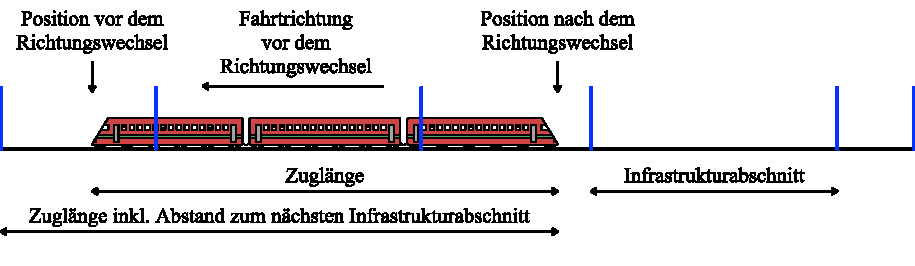
\includegraphics[width=\linewidth]{../images/vector/richtungsaenderung.pdf}
  \caption{Eigene Darstellung der Positionsbestimmung bei einem Richtungswechsel}
  \label{fig:richtungsaenderung}
\end{figure}
Damit die Fahrtrichtungsänderung ebenfalls funktioniert, wenn das Fahrzeug nicht am Ende eines \ac{infra}s steht, wird für die Ermittlung der neuen Position auf die Fahrzeuglänge der Abstand bis zum Ende \ac{infra}s addiert (siehe Abbildung \ref{fig:richtungsaenderung}). Über den aktuellen und die folgenden \acp{infra} (ermittelt durch die Funktion \textit{getNaechsteAbschnitte$($$)$}$^\ast$ (\textit{functions\_ebuef.php}), des aktuellen \ac{infra}s und der neuen Fahrtrichtung) wird iteriert und die Summe der Längen gebildet, bis die Fahrzeuglänge (zuzüglich des Abstands bis zum Ende des \ac{infra}s) überschritten wird. Der \ac{infra}, in dem die Fahrzeuglänge inkl. des Abstands zum ersten Mal überschritten wird, entspricht dem \ac{infra} der neuen Position.

Sollte die Länge aller nächsten Abschnitte inklusive des aktuellen Abschnitts in der Summe kleiner sein, als die Zuglänge inkl. dem Abstands bis zum Ende des Infra-Abschnitts, kann die neue Position nicht ermittelt werden und dem Fahrzeug wird eine Fehlermeldung übergeben, sodass das Fahrzeug nicht weiter fahren wird. Andernfalls wird die Richtung des Fahrzeugs in der Datenbank geändert und dem Fahrzeug mit der Funktion \textit{send\-Fahrzeugbefehl$($$)$}$^\ast$ (\textit{functions\_ebuef.php}) die Geschwindigkeit \mbox{-4 $km/h$} (entspricht einem Wendeauftrag) übergeben.

Bei einem \Gls{fahrtverlauf} kann es vorkommen, dass Fahrzeuge mit Fahrplan auf der Fahrt mehrere Betriebsstellen passieren. Damit dem Eintrag \textit{angekommen} dieser Betriebsstellen auch der Wert \textit{true} zugewiesen werden kann, wird überprüft, ob in den \Gls{echtzeitdaten} dem Eintrag \textit{live\_all\_targets\_reached} ein Wert zugewiesen ist. Dieser Eintrag enthält -- falls das Fahrzeug eine Betriebsstelle erreicht hat -- den Index der Betriebsstelle und weist der Betriebsstelle unter dem Eintrag \textit{angekommen} den Wert \textit{true} zu.

Wenn die letzten \Gls{echtzeitdaten} eines Fahrzeugs übermittelt wurden (\textit{live\_""target\_""reached} == \textit{true}) und das Fahrzeug dementsprechend zum Stehen gekommen ist, wird überprüft, wie sich das Fahrzeug als nächstes verhalten soll. Dafür wird zwischen vier Fällen (siehe Tabelle \ref{table:vierfaelle}) unterschieden.
\begin{table}
\begin{center}
\renewcommand{\arraystretch}{1.2}
\begin{tabular}{c|c|c}
 & Fährt jetzt ohne Fahrplan & Fährt jetzt nach Fahrplan \\ \hline
Fuhr davor ohne Fahrplan                 		&    1. Fall         & 2. Fall       \\ \hline
Fuhr davor nach Fahrplan                   		&    3. Fall         & 4. Fall       \\ 
\end{tabular}
\renewcommand{\arraystretch}{1}
\caption{Verhalten eines Fahrzeugs nach dem Erreichen des Ziels}
\label{table:vierfaelle}
\end{center}
\end{table}
Für die Überprüfung, ob sich der Fahrplan eines Fahrzeugs geändert hat, wird über die Funktion \textit{getFahrzeugZugIds$($$)$} (\textit{functions\_ebuef.php}) die aktuelle \Gls{zugid} abgefragt und mit der vorherigen verglichen. In dem \textbf{1. Fall} (alte und neue \Gls{zugid} haben beide den Wert \textit{null}) werden dem Fahrzeug keine neue Daten übergeben und ein neuer Fahrtverlauf wird versucht zu berechnen, sobald die \Gls{fahrstrasse} sich verändert hat. In dem \textbf{2.} und \textbf{4. Fall} wird die neue \Gls{zugid} dem Fahrzeug übergeben, der Eintrag \textit{operates\_on\_time\-table} auf \textit{true} gesetzt und die Funktionen \textit{get\-Fahr\-plan\-And\-Po\-sition\-For\-One\-Train$($$)$} (\textit{func\-tions.php}), \textit{add\-Stop\-sections\-For\-Time\-table$($$)$} (\textit{func\-tions.php}), \textit{calculate\-Next\-Sec\-tions$($$)$} (\textit{func\-tions\_fahrtverlauf.php}), \textit{check\-If\-Fahrstrasse\-Is\-Corrrect$($$)$} (\textit{func\-tions.php}) und \textit{calculate\-Fahrt\-ver\-lauf$($$)$} (\textit{func\-tions\-.php}) aufgerufen. Abgesehen von der ersten Funktion, werden diese Funktionen auch beim Start des Programms ausgeführt, welcher in Kapitel \ref{main_2} beschrieben wird. Die Funktion \textit{get\-Fahrplan\-And\-Position\-For\-One\-Train$($$)$} (\textit{func\-tions.php}) ähnelt der in Kapitel \ref{main_2} beschrieben Funktion \textit{pre\-pare\-Train\-For\-Ride$($$)$} (\textit{func\-tions.php}), fügt aber nur die Position und den Fahrplan hinzu, da alle anderen Daten schon eingelesen wurden. In dem \textbf{3. Fall} (die neu ermittelte \Gls{zugid} hat den Wert \textit{null}) wird der Eintrag \textit{operates\_on\_timetable} auf \textit{false} gesetzt und die Funktionen \textit{cal\-cu\-late\-Next\-Sec\-tions$($$)$} (\textit{func\-tions.php}) und \textit{cal\-cu\-late\-Fahrt\-ver\-lauf$($$)$} (\textit{func\-tions.php}) aufgerufen.
\subsection{Überprüfung nach einer Änderung der \Gls{fahrstrasse}}
Für die Überprüfung, ob sich die \Gls{fahrstrasse} der Züge verändert hat, wird in regelmäßigen Abständen die \Gls{fahrstrasse} der Fahrzeuge ermittelt und mit der aktuell hinterlegten \Gls{fahrstrasse} verglichen. Das Intervall, in dem diese Überprüfung stattfindet kann über die Variable \textit{\$timeCheckFahrstrasseInterval} (\textit{fahrzeugsteuerung.php}) festgelegt werden und ist standardgemäß auf 3 Sekunden festgelegt. Bei der Ermittlung und dem Vergleich der \Gls{fahrstrasse} wird für jedes Fahrzeug die Funktion \textit{compare\-Two\-Naechste\-Abschnitte$($$)$} (\textit{functions.php}) aufgerufen. Innerhalb dieser Funktion wird die in Kapitel \ref{main_2} erläutere Funktion \textit{calculateNextSections$($$)$} (\textit{functions.php}) aufgerufen, mit dem Unterschied, dass die ermittelten nächsten \acp{infra} inkl. der Längen und zulässigen Höchstgeschwindigkeiten nicht dem Fahrzeug hinterlegt werden, sondern lokal in der Funktion gespeichert. Damit die ermittelten Daten für ein Fahrzeug berechnet werden, aber nicht dem Fahrzeug hinterlegt werden, kann der Parameter \textit{\$writeResultToTrain} der Funktion \textit{calculateNextSections$($$)$} (\textit{functions.php}) (standardgemäß auf \textit{true} gesetzt) auf \textit{false} gesetzt werden. Sollte sich die \Gls{fahrstrasse} geändert haben, wird mit der Funktion \textit{check\-If\-Fahr\-strasse\-Is\-Corrrect$($$)$} (\textit{functions.php}) überprüft, ob die \Gls{fahrstrasse} dem Fahrplan (falls vorhanden) entspricht und im Anschluss die Funktion \textit{cal\-cu\-late\-Fahrt\-verlauf$($$)$} (\textit{functions.php}) aufgerufen.
\subsection{Neukalibrierung der Fahrzeugposition}  \label{main_5}
Für eine genau Fahrzeugsteuerung ist die aktuelle Position der Züge es­sen­zi­ell und muss während der Fahrt kalibriert werden, damit Ungenauigkeiten ausgeglichen werden können. Dafür werden die Daten aus der \textit{MySQL}-Tabelle \textit{fahrzeuge\_abschnitte} benötigt, welche durch die Abschnittsüberwachung ermittelt werden. Die Abschnittsüberwachung schreibt für jedes Fahrzeug den aktuellen \ac{infra} in die Datenbank, sobald der Zugkopf den Abschnitt befährt inklusive der aktuellen Zeit (\Gls{realzeit}). Für jedes Fahrzeug, welches durch die Übermittlung der \Gls{echtzeitdaten} in einen neuen \ac{infra} einfährt und seit der Einfahrt in den Abschnitt die Geschwindigkeit nicht verändert hat, wird die aktuelle Position neu ermittelt. Würde sich das Fahrzeug in einem \ac{infra} befinden und hätte seit der Einfahrt die Geschwindigkeit angepasst, könnte mit der Fahrzeugsteuerung die Position nicht neu berechnet werden, da nicht bekannt ist, welche Strecke das Fahrzeug seit der Einfahrt zurückgelegt hat. Aus diesem Grund wird, sobald das Fahrzeug nach den \Gls{echtzeitdaten} einen neuen Abschnitt befährt und aktuell nicht die Geschwindigkeit anpasst (\textit{live\_is\_speed\_change} == \textit{false}) dem Eintrag \textit{calibrate\_section\_one} der aktuelle \ac{infra} hinzugefügt und dem Eintrag \textit{calibrate\_section\_two} wird ebenfalls der aktuelle \ac{infra} hinzugefügt, wenn \textit{calibrate\_section\_one} ein Wert zugewiesen ist und dieser nicht dem aktuellen \ac{infra} der \Gls{echtzeitdaten} entspricht. Soabld das Fahrzeug seine Geschwindigkeit anpasst (\textit{live\_""is\_""speed\_""change} == \textit{true}), wird beiden Einträgen der Wert \textit{null} zugewiesen. Dadurch ist dem Eintrag \textit{calibrate\_section\_two} nur dann ein \ac{infra} zugewiesen, wenn das Fahrzeug in diesem seit der Einfahrt die Geschwindigkeit nicht verändert hat. Wenn dem Eintrag \textit{\$useRecalibration} aus der Datei \textit{global\_variables.php} der Wert \textit{true} zugewiesen ist, wird in regelmäßigen Abständen überprüft, ob eine Neukalibrierung möglich ist. Das Zeitintervall, in dem die Überprüfung stattfindet ist standardmäßig auf 3 Sekunden eingestellt, kann aber mittels der Variable \textit{\$timeCheckCalibrationInterval} (\textit{fahrzeugsteuerung.php}) angepasst werden.

Für die Neukalibrierung wird die Funktion \textit{getCalibratedPosition$($$)$} (\textit{functions.php}) (Code-Beispiel \ref{lst:getCalibratedPosition}) aufgerufen, welche als Rückgabewert die aktuelle relative Position und den aktuellen \ac{infra} zurückgibt.
\begin{figure}
\begin{lstlisting}[caption={\textit{getCalibratedPosition$($$)$} (\textit{functions\_db.php})},captionpos=b,label={lst:getCalibratedPosition}]
// Kalibriert die Position des Fahrzeugs neu anhand der Daten in der Tabelle
// 'fahrzeuge_abschnitte'
function getCalibratedPosition ($id, $speed) {
	global $cacheFahrzeugeAbschnitte;
	$DB = new DB_MySQL();
	$positionReturn = $DB->select("SELECT `".DB_TABLE_FAHRZEUGE_ABSCHNITTE."`.`infra_id`,`".DB_TABLE_FAHRZEUGE_ABSCHNITTE."`.`unixtimestamp` FROM `".DB_TABLE_FAHRZEUGE_ABSCHNITTE."` WHERE `".DB_TABLE_FAHRZEUGE_ABSCHNITTE."`.`fahrzeug_id` = $id")[0];
	unset($DB);
	if (in_array($id, array_keys($cacheFahrzeugeAbschnitte))) {
		if ($positionReturn->unixtimestamp == $cacheFahrzeugeAbschnitte[$id]["unixtimestamp"]) {
			return array("possible" => false);
		}
	}
	$timeDiff = time() - $positionReturn->unixtimestamp;
	$position = ($speed / 3.6) * $timeDiff;
	return array("section" => $positionReturn->infra_id, "position" => $position);
}
\end{lstlisting}
\end{figure}

Sollte die ermittelte Position innerhalb des \ac{infra}s größer als die Länge des \ac{infra}s sein, welche in dem Array \textit{\$cacheInfraLaenge} abgespeichert ist, wird die Neukalibrierung nicht durchgeführt. Der aktuelle \ac{infra} wird aus der Tabelle \textit{fahrzeuge\_abschnitte} der \textit{MySQL}-Datenbank geladen und durch die aktuelle Geschwindigkeit des Fahrzeugs und die Differenz der Zeit zwischen dem Einfahren in den \ac{infra} und der aktuellen Zeit wird die relative Position innerhalb des \ac{infra}s berechnet.
\begin{equation*}
\textrm{relative Position} = \textrm{Geschwindigkeit} \cdot \textrm{Zeitdifferenz (aktuelle Zeit} - \textrm{Zeit des Einfahrens)}
\end{equation*}
\subsection{Ermittlung von neuen Fahrzeugen im eingleisigen Netz} \label{main_6}
Die Fahrzeugsteuerung betrachtet neben den Fahrzeugen, welche sich schon zu Beginn des Programmstarts im eingleisigen Netz befinden auch alle Fahrzeuge, die nach dem Programmstart hinzugefügt werden. Für alle Fahrzeuge, die beim Start des Programms erkannt werden, wird in dem Array \textit{\$allTrainsOnTheTrack} die zugehörige Adresse gespeichert (\textit{find\-Trains\-On\-The\-Tracks$($$)$}) (\textit{functions.php}). Für die Überprüfung, ob Fahrzeuge entfernt wurden oder neu hinzugekommen sind, wird die Funktion \textit{up\-date\-All\-Trains\-On\-The\-Track$($$)$} (\textit{functions.php}) verwendet. Diese Funktion wird -- wie die Neukalibrierung in Kapitel \ref{main_5} -- alle 3 Sekunden ausgeführt. Bei dem Aufruf der Funktion werden alle Fahrzeuge geladen, denen in der \textit{fma}-Tabelle aus der Datenbank ein \ac{infra} zugeordnet ist und mit dem Array \textit{\$allTrainsOnTheTrack} verglichen. Fahrzeugadressen, die nicht in dem Array hinterlegt sind, werden in dem Rückgabe-Array unter dem Eintrag \textit{new} zurückgegeben und alle Fahrzeugadressen, die in dem Array enthalten sind, aber bei dem Aufruf der Funktion keinem \ac{infra} zugeordnet sind, werden in dem Rückgabe-Array unter dem Eintrag \textit{removed} zurückgegeben. Nach dem Aufruf der Funktion, werden für alle neuen Fahrzeuge die Funktion \textit{pre\-pare\-Train\-For\-Ride$($$)$} (\textit{func\-tions.php}), \textit{add\-Stop\-sec\-tions\-For\-Time\-table$($$)$} (\textit{func\-tions.php}), \textit{cal\-culate\-Next\-Sec\-tions$($$)$} (\textit{func\-tions.php}), \textit{check\-If\-Train\-Reached\-Halte\-punkt$($$)$} (\textit{func\-tions.php}), \textit{check\-If\-Fahr\-strasse\-Is\-Corrrect$($$)$} (\textit{func\-tions.php}) und \textit{calculate\-Fahrt\-ver\-lauf$($$)$} (\textit{func\-tions\-.php}) aufgerufen (siehe Kapitel \ref{main_2} und \ref{main_3}). Alle entfernten Fahrzeuge werden aus dem Array \textit{\$allUsedTrains} entfernt und somit nicht mehr von der Fahrzeugsteuerung beachtet. 
\subsection{Fehlerbehebung von Fahrzeugen} \label{main_7}
Wenn es bei einem Fahrzeug zu einem Konflikt kommt, der eine Steuerung des Fahrzeugs verhindert, wird dem Fahrzeug eine Fehlermeldungs-ID unter dem Eintrag \textit{error} in dem \textit{\$allUsedTrains} zugewiesen. Fahrzeuge, denen eine Fehlermeldung zugeordnet wurde, werden ab diesem Zeitpunkt nicht weiter von der Fahrzeugsteuerung berücksichtigt. Für das Erkennen von Fahrzeugen mit Fehlermeldungen, wird in regelmäßigen Zeitintervallen (\textit{\$time\-Check\-All\-Train\-Sta\-tus\-Inter\-val}) die Funktion \textit{showErrors$($$)$} (\textit{functions.php}) aufgerufen, welche die Fehlermeldungen aller Fahrzeuge ausgibt (Code-Beispiel \ref{lst:showErrors}).
\begin{figure}
\begin{lstlisting}[caption={\textit{showErrors$($$)$} (\textit{functions.php})},captionpos=b,label={lst:showErrors}]
// Gibt für alle Fahrzeuge die vorhanden Fehlermeldungen an.
function showErrors() {

	global $allUsedTrains;
	global $trainErrors;

	$foundError = false;
	echo "Hier werden für alle Züge mögliche Fehler angezeigt:\n\n";

	foreach ($allUsedTrains as $trainIndex => $trainValue) {
		if (sizeof($trainValue["error"]) != 0) {
			$foundError = true;
			echo "Zug ID: ", $trainValue["id"], "\n";
			$index = 1;

			foreach ($trainValue["error"] as $error) {
				echo "\t", $index, ". Fehler:\t", $trainErrors[$error], "\n";
				$index++;
			}

			echo "\n";
		}
	}

	if (!$foundError) {
		echo "Keiner der Züge hat eine Fehlermeldung.\n";
	}
}
\end{lstlisting}
\end{figure}
Für das Beheben einer Fehlermeldung muss das Fahrzeug händisch vom Schienennetz genommen werden, gewartet werden, bis die Fahrzeugsteuerung das Entfernen registriert hat und das Fahrzeug wieder händisch auf das Schienennetz gesetzt werden.

Die möglichen Fehlermeldungen sind in dem Array \textit{\$trainErrors} gespeichert und können um beliebig viele weitere Fehlermeldungen ergänzt werden. Für die Implementierung einer neuen Fehlermeldung muss lediglich die Fehlermeldungs-ID (Index der Fehlermeldung in dem \textit{\$trainErrors}-Array) dem Eintrag \textit{error} aus dem \textit{\$allUsedTrains}-Array hinzugefügt werden, sobald der Konflikt in der Fahrzeugsteuerung auftritt.
\begin{table}
\begin{center}
\renewcommand{\arraystretch}{1.2}
\begin{tabular}{c|c}
Fehlermeldungs-ID & Beschreibung  \\ \hline
0 &    \makecell{Fahrtrichtung des Fahrzeugs musste geändert werden\\und die Positionsbestimmung war nicht möglich} \\\hline
1              &    \makecell{In der Datenbank ist für das Fahrzeug\\keine Zuglänge angegeben}             \\ \hline
2         &    \makecell{In der Datenbank ist für das Fahrzeug\\keine v\_max angegeben}             \\ \hline
3        &   \makecell{Das Fahrzeug musste eine\\Gefahrenbremsung durchführen}          \\ 
\end{tabular}
\renewcommand{\arraystretch}{1}
\caption{Übersicht der Fehlermeldungen}
\label{table:fehlertabelle}
\end{center}
\end{table}
In Tabelle \ref{table:fehlertabelle} sind alle Fehlermeldungen aufgelistet, welche aktuell in der Fahhrzeugsteuerung implementiert sind.
%\linebreak[4] -> behält blocksatz bei







































